\chapter{涵道风扇式无人机系统构成及建模}

为方便检验本文的研究成果,自主搭建了一架DFUAV试验样机。本章首先简要介绍试验样机的结构组成和机载航电系统,然后重点是对DFUAV进行系统建模,这将是后续进行飞行控制算法设计的基础。物体的相对运动离不开其所处的参考坐标系,因此在建模之前将先介绍本文所使用的坐标系描述方法以及DFUAV的姿态表示方法。在建模分析中,为简化模型复杂度便于控制算法的设计,有必要假设无人机是刚体。然后采用在刚体上应用广泛的牛顿-欧拉方法推导出DFUAV的刚体运动学模型和动力学模型,得到飞行控制的刚体模型。最后分析了作用在涵道上的力与力矩并作出总结。
% DFUAV的系统建模中各变量定义标准主要参考文献\parencite{杨一栋2019直升机飞行控制},并为了表示方便,避免混淆,对部分变量的表示作略微修改。

\section{试验样机的系统组成}

\subsection{主要结构介绍}

自主搭建的DFUAV试验样机的实物及主要结构如图\ref{DFUAV}所示。类似大部分无人机,DFUAV也有电子仓、电池、电调、电机和螺旋桨等组成部件。电子仓中放置了飞行控制系统的硬件,电池是DFUAV的能量来源,电调、电机和螺旋桨共同组成了DFUAV的动力系统。不同于常规旋翼无人机,DFUAV的螺旋桨由涵道体包裹,用于提升拉力效率和安全性。在螺旋桨下方的滑流区安装有固定气动面用于提供反扭距,最下方安装了四个控制舵面用于提供DFUAV的三维力矩。

\begin{figure}[htbp]
	\centering
    \subfloat[试验样机]
		{
\includegraphics[scale=0.85]{Fig/DFUAV.jpg}
		\label{试验样机}}
        \subfloat[结构组成示意]{
		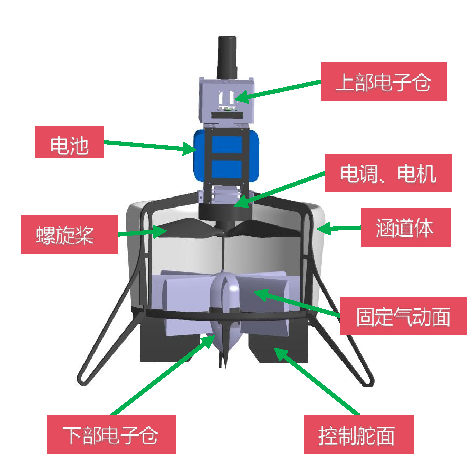
\includegraphics[scale=1]{Fig/涵道结构.pdf}
		\label{主要结构组成}}
        \caption{试验样机及结构组成}\label{DFUAV}
\end{figure}

\subsection{机载航电系统}

图\ref{主要结构组成}中的上部电子仓和下部电子仓共同构成了DFUAV的机载航电系统,掌控着飞行的各个环节,系统内部主要包括微控制器、各种传感器、通信链路等部分。下面对这些部分进行简要介绍:

(1)微控制器(MCU)

    作为DFUAV飞行控制系统的核心处理器,MCU承担着多传感器数据融合与实时决策的关键任务。本系统选用意法半导体公司生产的基于ARM架构的STM32F767系列MCU,其工作频率高达216MHz,通信接口丰富(包括UART/USART、SPI、I2C、CAN等)以及2MB的闪存和512KB的静态随机存储器。其高性能低功耗的特点十分适用于DFUAV的控制。

(2)惯性测量单元(IMU)

    IMU用于测量无人机的加速度和角速度,其输出的数据被用于实时解算无人机的姿态。本系统选用了InvenSense公司的ICM-20602六轴IMU,内部集成了三轴陀螺仪和三轴加速度计。ICM-20602具有高量程($\pm16g$)、大缓冲区(1KB的FIFO)和高精度(误差$\pm1\%$)等特点,并且可以以10MHz的SPI接口或者400kHz的I2C接口输出数据。

(3)磁力计

    磁力计固连在机体上用于测量当前位置的地磁感应强度,其输出的数据结合IMU数据被用于实时解算无人机的航向。本系统选用意法半导体公司的LSM303D系列磁力计,由于测量的数据易受到外界磁场干扰,尤其是电池放电过程中产生的磁场,所以磁力计被安装在远离电池的下部电子仓内。

(4)卫星定位模块

    卫星定位模块用于接收多颗卫星信号来获取无人机的位置和速度等信息。本系统选用了瑞士u-blox公司的ZED-F9P-04B的高精度GPS卫星定位模块,该模块收敛时间快并且方便集成实时动态载波相位差分技术(RTK)实现厘米级的定位精度。
    
(5)气压计

    气压计用于测量当前位置的大气压强并进一步解算出海拔高度。本系统选用的英飞凌公司的DPS368压力传感器,该产品自带防风外壳,基于电容式传感原理在温度变化时依然能保持高精度($\pm0.02m$),可以在恶劣环境中使用。

(6)无线数据传输模块

    无线数据传输模块用于地面站与飞机之间的无线通信,包括由地面站发送给飞机的控制指令和飞机发送到地面站的状态信息等,本方案选用Microhard的hp840无线调制解调器,支持840-845MHz的跳频或定频工作以及理想情况下160公里的传输距离。

在飞行控制周期内,MCU首先首先完成多个传感器设备的协同启动与自检流程,然后通过外设接口读取IMU、磁力计、GPS、气压计等传感器的数据。接下来通过滤波方法对数据进行平滑去噪等处理,并且通过导航算法融合数据解算出无人机的位置、速度、姿态和角速度等状态信息。借助多频段无线数传模块构建的低延迟通信链路,无人机不仅以50Hz刷新率向地面站传输飞行状态遥测数据包,同时实时接收包含航点指令、模式切换、紧急制动等要素的上行控制帧。控制指令与实时飞行状态参数共同输入至飞行控制决策层,经过飞行控制算法处理后,计算出给到执行机构(电机和舵机)的指令,从而实现对飞行器六自由度运动的闭环控制。


\section{坐标系和姿态表示方法}

考虑到无人机的位置变化与姿态变化,基于地面坐标系($\boldsymbol{O}_e-\boldsymbol{X}_e\boldsymbol{Y}_e\boldsymbol{Z}_e $)和机体坐标系(${\boldsymbol{O}_b}-{\boldsymbol{X}_b}{\boldsymbol{Y}_b}{\boldsymbol{Z}_b}$)的多坐标系表示法被广泛应用于无人机的运动分析与控制系统设计中。

% \begin{enumerate}[topsep = 0 pt, itemsep= 0 pt, parsep=0pt, partopsep=0pt, leftmargin=44pt, itemindent=0pt, labelsep=6pt, label=(\arabic*)]
% \item 地面坐标系
(1)地面坐标系

地面坐标系的原点$\boldsymbol{O}_e$可以是地平面上的任意一点,一般定义为无人机的起飞点。三轴方向分别为$\boldsymbol{O}_e-\boldsymbol{X}_e$轴在地平面内指向地理正北方向(N),$\boldsymbol{O}_e-\boldsymbol{Y}_e$轴在地平面内指向地理正东方向(E),$\boldsymbol{O}_e-\boldsymbol{Z}_e$轴按照右手定则,垂直于地面指向地心,方向向下(D)。因此地面坐标系也被称为北东地(NED)坐标系,该坐标系与地球固连。

% \item 机体坐标系
(2)机体坐标系

机体坐标系与无人机的机体固连,其原点$\boldsymbol{O}_b$定义为无人机的重心位置。三轴方向分别为$\boldsymbol{O}_b-\boldsymbol{X}_b$轴在无人机对称平面内指向人为定义的机头方向,$\boldsymbol{O}_b-\boldsymbol{Z}_b$轴在无人机对称平面内垂直于$\boldsymbol{O}_b-\boldsymbol{X}_b$轴向下为正,$\boldsymbol{O}_b-\boldsymbol{Y}_b$轴按照右手定则与$\boldsymbol{X}_b-\boldsymbol{O}_b-\boldsymbol{Z}_b$平面垂直,沿着机身的右侧方向向右为正。
% \end{enumerate}

地面坐标系和机体坐标系定义如图\ref{坐标系}所示。同一个物理量在不同的坐标系中有不同的大小和方向,为便于区分,在全文中统一使用上标$(.)^{e}$与$(.)^{b}$表示同一个物理量分别在地面坐标系和机体坐标系下的表示。

在地面坐标系下采用惯性导航系统、GPS导航等方式,无人机的位置和速度等运动状态可以方便直观地映射到地理空间中。这种方式使得无人机的飞行轨迹与实际地理位置紧密相关,以便进行飞行路线规划和轨迹优化。无人机的重心相对于地面坐标系的位置矢量在地面坐标系下表示为$\boldsymbol{P}^{e}=[{x}^{e} \quad {y}^{e} \quad {z}^{e}]^{T}$,机体重心沿着地面坐标系的速度矢量在地面坐标系下表示为$\boldsymbol{V}^{e}=[{v}^{e}_{x} \quad {v}^{e}_{y} \quad {v}^{e}_{z}]^{T}$,机体重心相对于地面坐标系的速度矢量在机体坐标系下表示为$\boldsymbol{V}^{b}=[{u} \quad {v} \quad {w}]^{T}$。

地面坐标系与机体坐标系的旋转变化关系体现了无人机的姿态变化,无人机常用的姿态描述方法有欧拉角、旋转矩阵和四元数等方式。其中欧拉角表示方法因物理意义明确,表示直观,所以被广泛采用。但因其奇异性问题\cite{全权2018多旋翼飞行器设计与控制},欧拉角表示法在一些特殊场景的使用下受到制约(如横滚角或者俯仰角为$\pm90^{\circ}$的情况)。考虑到本研究在姿态控制中,由于输入姿态指令和输出舵面角度的约束,不会出现上述奇异情况,所以本文采用欧拉角来描述无人机的姿态。根据欧拉定理,地面坐标系按照某个固定点经过三次基本旋转可以得到机体坐标系。由于旋转运动与坐标系原点的位置无关,所以为便于理解,将地面坐标系的原点与机体坐标系原点重合(即$\boldsymbol{O}_e=\boldsymbol{O}_b$),如图\ref{欧拉角}所示。在三次基本旋转中,旋转轴是待转动坐标系的某一轴,旋转的角度即为欧拉角。由于姿态旋转矩阵可以表示为三次基本旋转的乘积,所以与旋转顺序密切相关。由于本研究不会出现奇异问题,所以本文采用常用的‘Z-Y-X’的旋转顺序的欧拉角表示法。

\begin{figure}[htbp]
	\centering
	\begin{minipage}[c]{0.5\textwidth}
		\centering
		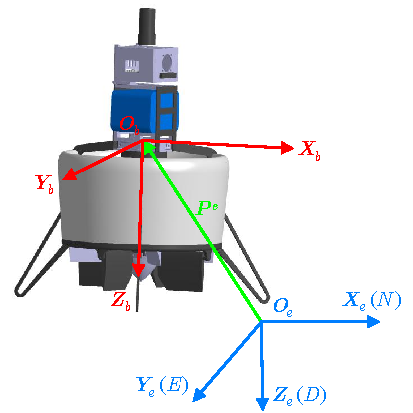
\includegraphics[scale=1]{Fig/坐标系.pdf}
		\caption{\label{坐标系}地面坐标系与机体坐标系定义}
	\end{minipage}%
    \begin{minipage}[c]{0.5\textwidth}
		\centering
		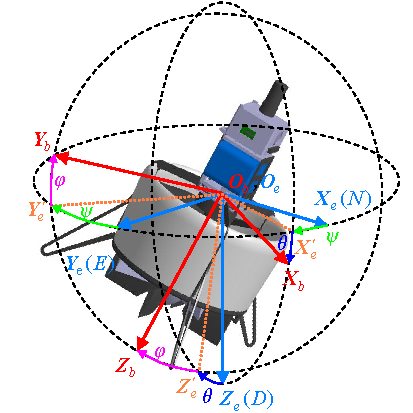
\includegraphics[scale=1]{Fig/欧拉角.pdf}
		\caption{\label{欧拉角}‘Z-Y-X’欧拉角的定义}
	\end{minipage}%
\end{figure}

在图\ref{欧拉角}中,地面坐标系$\boldsymbol{O}_e-\boldsymbol{X}_e\boldsymbol{Y}_e\boldsymbol{Z}_e$首先围绕$\boldsymbol{Z}_e$轴旋转偏航角$\psi$,向右偏航为正方向。此时$\boldsymbol{X}_e$轴旋转至$\boldsymbol{X}_e^{'}$轴,$\boldsymbol{Y}_e$轴旋转至$\boldsymbol{Y}_e^{'}$轴,$\boldsymbol{Z}_e$轴保持不变;
然后临时坐标系$\boldsymbol{O}_e-\boldsymbol{X}_e^{'}\boldsymbol{Y}_e^{'}\boldsymbol{Z}_e$围绕$\boldsymbol{Y}_e^{'}$轴旋转俯仰角$\theta$,上仰为正方向。此时$\boldsymbol{X}_e^{'}$轴旋转至$\boldsymbol{X}_b$轴,与机体系保持一致,$\boldsymbol{Z}_e$轴旋转至$\boldsymbol{Z}_e^{'}$轴,$\boldsymbol{Y}_e^{'}$轴保持不变;
最后临时坐标系$\boldsymbol{O}_e-\boldsymbol{X}_b\boldsymbol{Y}_e^{'}\boldsymbol{Z}_e^{'}$围绕$\boldsymbol{X}_b$轴旋转滚转角$\varphi$,向右滚转为正方向。此时$\boldsymbol{Y}_e^{'}$轴旋转至$\boldsymbol{Y}_b$轴,$\boldsymbol{Z}_e^{'}$轴旋转至$\boldsymbol{Z}_b$轴,均与机体系保持一致。

三次基本旋转的角度分别为$\psi$、$\theta$、$\varphi$,定义其对应的旋转矩阵分别为$\boldsymbol{R}_\psi,\boldsymbol{R}_\theta,\boldsymbol{R}_\varphi\in{SO(3)}$,其中$SO(3)=\{\boldsymbol{R}\in\mathbb{R}^{3\times3}|\boldsymbol{R}\boldsymbol{R}^T=I,|\boldsymbol{R}|=1\}$。
\begin{equation}
    \begin{aligned} %表示公式编号上下居中
\boldsymbol{R}_\psi=\begin{bmatrix}\cos\psi & \sin\psi & 0 \\-\sin\psi & \cos\psi & 0 \\0 & 0 & 1\end{bmatrix},\boldsymbol{R}_\theta=\begin{bmatrix}\cos\theta & 0 & -\sin\theta \\0 & 1 & 0 \\\sin\theta & 0 & \cos\theta\end{bmatrix},\boldsymbol{R}_\varphi=\begin{bmatrix}1 & 0 & 0\\0 & \cos\varphi & \sin\varphi \\0 & -\sin\varphi & \cos\varphi\end{bmatrix}\label{eq_1}
    \end{aligned}
\end{equation}

为表述方便,定义如下单位向量:
\begin{equation}
    \begin{aligned}
\boldsymbol{e}_1=\begin{bmatrix}1 \\0 \\0\end{bmatrix},
\quad\boldsymbol{e}_2=\begin{bmatrix}0 \\1 \\0\end{bmatrix},
\quad\boldsymbol{e}_3=\begin{bmatrix}0 \\0 \\1\end{bmatrix}\label{eq_2}
    \end{aligned}
\end{equation}

机体姿态的欧拉角表示为$\boldsymbol{\eta}=[\varphi \quad \theta \quad \psi]^T$,对应的姿态变化率为$\boldsymbol{\dot{\eta}}=[\dot{\varphi} \quad \dot{\theta} \quad \dot{\psi}]^T$。定义沿机体轴的旋转角速度为$\boldsymbol{\omega}^b=[p \quad q \quad r]^T$,那么旋转角速度与机体姿态变化率的关系如下\cite{ducard2009fault}:
\begin{equation}
    \boldsymbol\omega^{b}=\dot{\psi}\boldsymbol{R}_{\varphi} \boldsymbol{R}_{\theta} \boldsymbol{e}_{3}+\dot{\theta}\boldsymbol{R}_{\varphi}\boldsymbol{e}_{2}+\dot{\varphi}\boldsymbol{e}_{1}\label{eq_3}
\end{equation}
结合式\eqref{eq_1}、式\eqref{eq_2}和式\eqref{eq_3},得到:
\begin{equation}
    \begin{gathered}
    \boldsymbol\omega^{b}=
    \begin{bmatrix}
    1 & 0 & -\sin\theta \\
    0 & \cos\varphi & \sin\varphi\cos\theta \\
    0 & -\sin\varphi & \cos\varphi\cos\theta
    \end{bmatrix}
    \boldsymbol{\dot{\eta}}
    \\
    \Leftrightarrow\dot{\boldsymbol{\eta}}=\boldsymbol{Q}\boldsymbol{\omega}^b,\quad\boldsymbol{Q}\triangleq
    \begin{bmatrix}
        1 & \sin\varphi\tan\theta & \cos\varphi\tan\theta \\
        0 & \cos\varphi & -\sin\varphi \\
        0 & \dfrac{\sin\varphi}{\cos\theta} & \dfrac{\cos\varphi}{\cos\theta}
        \end{bmatrix}
    \label{eq_4}
    \end{gathered}
\end{equation}

进一步地,在欧拉角‘Z-Y-X’的旋转顺序下,由机体坐标系到地面坐标系的旋转矩阵$\boldsymbol{R}^e_b$可以表示为:
\begin{equation}
    \begin{aligned}
    \boldsymbol{R}_{b}^{e} & =(\boldsymbol{R}_{e}^{b})^T =(\boldsymbol{R}_\varphi\boldsymbol{R}_\theta\boldsymbol{R}_\psi)^T \\
     & =
    \begin{bmatrix}
    \cos{\theta}\cos{\psi} & \sin{\varphi}\sin{\theta}\cos{\psi}-\cos{\varphi}\sin{\psi} & \cos{\varphi}\sin{\theta}\cos{\psi} + \sin{\varphi}\sin{\psi}
    \\ 
    \cos{\theta}\sin{\psi} & \sin{\varphi}\sin{\theta}\sin{\psi} + \cos{\varphi}\cos{\psi} & \cos{\varphi}\sin{\theta}\sin{\psi} - \sin{\varphi}\cos{\psi}
    \\
    -\sin{\theta} & \sin{\varphi}\cos{\theta} & \cos{\varphi}\cos{\theta}
    \end{bmatrix}
    \label{eq_5}
    \end{aligned}
\end{equation}

\section{飞行控制刚体模型}

DFUAV的建模过程需要在准确性与实用性之间找到合适的平衡,确保不会过于复杂而增加控制算法设计的难度和计算资源的开销,同时也不至于过于简单而与实际情况相差甚远。因此,在建模过程中假设DFUAV是刚体,并且假设DFUAV在飞行过程中其质量和转动惯量(机体坐标系下)保持不变。基于这种假设,DFUAV的刚体运动学和动力学模型可以通过牛顿-欧拉方法推导得到。

\subsection{刚体运动学模型}

运动学模型用于描述无人机在三维空间中的位置和姿态随时间变化的关系,不涉及力与力矩的分析。六自由度DFUAV的刚体运动学模型包括三自由度的位置运动学模型和三自由度的姿态运动学模型。在地面坐标系下,位置运动学模型可以表示为:$\boldsymbol{\dot{P}}^{e} = \boldsymbol{V}^{e}$。三自由度的姿态运动学模型分为欧拉角模型、旋转矩阵模型和四元数模型三种。在机体系下,根据式\eqref{eq_4},可以得到使用欧拉角模型表示三自由度的姿态运动学为$\dot{\boldsymbol{\eta}}=\boldsymbol{Q}\boldsymbol{\omega}^b$。

因此,六自由度的DFUAV刚体运动学模型可以表示为:
\begin{equation}
    \begin{aligned}
    \boldsymbol{\dot{P}}^{e} &= \boldsymbol{V}^{e} \\
    \dot{\boldsymbol{\eta}}&=\boldsymbol{Q}\boldsymbol{\omega}^b
    \end{aligned}
    \label{eq_6}
\end{equation}

\subsection{刚体动力学模型}

DFUAV的刚体动力学模型包括位置动力学模型和姿态动力学模型,动力学模型是描述无人机在三维空间中运动行为的数学模型,该模型主要基于牛顿第二定律和角动量定理推导,用于分析无人机在受力、力矩、环境扰动等因素共同作用下的运动行为。但是该定律仅在惯性系下成立,考虑到DFUAV的在运动时,地球自转对其的影响相对不显著,并且从局部来看,地面近似平坦,因此将地面坐标系假设为惯性系是合理的。

假设DFUAV受到的力包括重力和除重力之外的合外力作用$\boldsymbol{F}^b$,为下文受力分析方便,此处$\boldsymbol{F}^b\in\mathbb{R}^{3\times1}$表示在机体系下受到的除重力之外的合外力。那么根据牛顿第二定律可以得到:
\begin{equation}
    \begin{gathered}
    \boldsymbol{R}_b^e\boldsymbol{F}^b + mg\boldsymbol{e}_3 = m\dfrac{d({\boldsymbol{V}}^e)}{dt}
    \\
    \Leftrightarrow\dot{\boldsymbol{V}}^e=\dfrac{1}{m}\boldsymbol{R}_b^e\boldsymbol{F}^b + g\boldsymbol{e}_3 
    \label{eq_7}
    \end{gathered}
\end{equation}
其中$m$表示DFUAV的总质量,$g$表示当地的重力加速度。

姿态动力学模型由角动量定理描述:
\begin{equation}
    \begin{gathered}
    \boldsymbol{M}^{b}=\dfrac{d\boldsymbol{L}^{b}}{dt} - {\boldsymbol{L}^{b}}\times{\boldsymbol\omega^{b}},\quad \boldsymbol{L}^{b}=\boldsymbol{J}^{b}\boldsymbol\omega^{b}
    \\
    \Leftrightarrow\boldsymbol{\dot{\omega}}^b=(\boldsymbol{J}^b)^{-1}(\boldsymbol{M}^b+\boldsymbol{J}^b\boldsymbol{\omega}^b\times\boldsymbol{\omega}^b)
    \label{eq_8}
    \end{gathered}
\end{equation}
其中$\boldsymbol{M}^{b}\in\mathbb{R}^{3\times1}$表示DFUAV在机体系下受到的合外力矩,$\boldsymbol{L}^{b}\in\mathbb{R}^{3\times1}$表示DFUAV在机体系下总的角动量,‘$\times$’表示向量叉乘运算。$\boldsymbol{J}^{b}\in\mathbb{R}^{3\times3}$表示DFUAV在机体系中的转动惯量矩阵,其在机体系下是一个常量。根据图\Ref{DFUAV},可以看出本文研究的DFUAV呈现对称的几何结构,故本文建模过程中认为$\boldsymbol{J}^{b}$近似为一个对角矩阵,即
\begin{equation}
    \boldsymbol{J}^b=\begin{bmatrix}
        J_{x} & 0 & 0 \\
        0 & J_{y} & 0 \\
        0 & 0 & J_{z}
        \end{bmatrix}
    \label{eq_9}
\end{equation}

类似地,在机体系下可以更加直观地表示姿态动力学模型中相关变量,并且便于下文对力矩的分析,其中${\boldsymbol{L}^{b}}\times{\boldsymbol\omega^{b}}$部分分量表示由惯性系旋转到机体系产生的影响。

综合上述分析,可以得到DFUAV的飞行控制刚体模型:
\begin{equation}
    \left\{
    \begin{aligned}
        \boldsymbol{\dot{P}}^{e} &= \boldsymbol{V}^{e} \\
        \dot{\boldsymbol{V}}^e&=\dfrac{1}{m}\boldsymbol{R}_b^e\boldsymbol{F}^b + g\boldsymbol{e}_3 \\
        \dot{\boldsymbol{\eta}}&=\boldsymbol{Q}\boldsymbol{\omega}^b \\
        \boldsymbol{\dot{\omega}}^b&=(\boldsymbol{J}^b)^{-1}(\boldsymbol{M}^b+\boldsymbol{J}^b\boldsymbol{\omega}^b\times\boldsymbol{\omega}^b)
    \end{aligned}
    \right.
    \label{eq_10}
\end{equation}

\section{力与力矩分析}

对作用于DFUAV上的力与力矩进行分析是为了对控制算法的设计提供依据,明确其内在机理可以更好地分析运动特性。根据式\eqref{eq_10},DFUAV受到的除重力作用的合外力在机体系下表示为$\boldsymbol{F}^b$,受到的合外力矩在机体系下表示为$\boldsymbol{M}^b$。进一步地,$\boldsymbol{F}^b$和$\boldsymbol{M}^b$可以被分解为:
\begin{equation}
    \left\{
    \begin{aligned}
        \boldsymbol{F}^b&=\boldsymbol{F}_{fan}^b+\boldsymbol{F}_{aero}^b+\boldsymbol{F}_{duct}^b+\boldsymbol{F}_{vane}^b \\
        \boldsymbol{M}^b&=\boldsymbol{M}_{fan}^b+\boldsymbol{M}_{aero}^b+\boldsymbol{M}_{duct}^b+\boldsymbol{M}_{vane}^b+\boldsymbol{M}_{gyro}^b+\boldsymbol{M}_{flap}^b
    \end{aligned}
\right.
\label{eq_11}
\end{equation}
其中$\boldsymbol{F}_{fan}^b$和$\boldsymbol{M}_{fan}^b$表示由于涵道风扇旋转而产生的总的拉力和扭矩,$\boldsymbol{F}_{aero}^b$和$\boldsymbol{M}_{aero}^b$表示由于机身空气阻力产生的气动力和力矩,$\boldsymbol{F}_{duct}^b$和$\boldsymbol{M}_{duct}^b$表示作用于涵道环翼上的气动力与力矩,$\boldsymbol{F}_{vane}^b$和$\boldsymbol{M}_{vane}^b$表示由于涵道底部的控制舵面运动与风扇滑流相互作用而产生的力和力矩,$\boldsymbol{M}_{gyro}^b$表示由于涵道风扇的旋转而产生的陀螺力矩,$\boldsymbol{M}_{flap}^b$表示位于涵道底部的固定气动面于风扇滑流相互作用而产生的扭矩。下面将对各力与力矩的作用机理进行逐一分析。

\subsection{涵道风扇动力学}

涵道风扇是安装在圆形涵道内的螺旋桨,旋翼模型的研究主要基于基本动量理论和叶素理论。由于涵道入口边缘的吸力效应和出口处较高的静压的共同作用,相比于开放式的螺旋桨,在相同的功率下,涵道风扇具有更出色的静态性能。

可以使用动量理论进行悬停情况下的分析,在相同的功率条件下,推力增益可以描述为扩张比的函数:
\begin{equation}
    \dfrac{\boldsymbol{F}_{fan}^b}{\boldsymbol{F}_{prop}}={\sqrt[3]{2\Lambda}}
    \label{eq_12}
\end{equation}
其中$\boldsymbol{F}_{fan}^b$是由于涵道风扇旋转产生的总拉力,设其标量表示为$T_{fan}$。$T_{fan}$可以分为两部分:涵道风扇旋转产生的拉力$T_{p}$和侧风与涵道风扇抽吸作用产生的侧向拉力$T_{l}$。$\boldsymbol{F}_{prop}$表示传统开放式螺旋桨产生的拉力,$\Lambda$是扩张比。由式\eqref{eq_12}可以看出,扩张比大于0.5时,涵道风扇的推力增益大于1,即涵道风扇比开放式旋翼的推力效率更高。更详尽的分析可以在\parencite{pereiraHoverWindtunnelTesting2008}中找到。

% 据此定义涵道拉力分配系数:
% \begin{equation}
%     \lambda=\dfrac{T_{p}}{T_{fan}}=\dfrac{T_{p}}{T_{p}+T_{l}}
%     \label{eq_13}
% \end{equation}

% 由于涵道的遮挡作用,涵道出口的气流基本保持轴向流动,沿着轴线方向喷射出去,如图所示。假设空气密度为$\rho$,气流在未受到涵道风扇影响前的速度和压强分别为$V_0$和$p_0$,气流在逼近涵道风扇上表面时的速度增加为$V_1$同时压强减小为$p_1$。忽略风扇的厚度,气流通过风扇到下表面即将进入滑流区时,由于气流速度连续不可突变,所以认为气流速度保持$V_2=V_1$,但压强增加为$p_1+\Delta p$。气流进入滑流区后,速度进一步增大为$V_e$,压强恢复到来流状态$p_0$。在涵道风扇的上下表面分别应用伯努利方程:

% \noindent 上表面
% \begin{equation}
%         p_0+\frac{1}{2}\rho V_0^2=p_1+\frac{1}{2}\rho V_1^2
%     \label{eq_14}
% \end{equation}
% 下表面
% \begin{equation}
%     p_1+\Delta p+\frac{1}{2}\rho V_2^2=p_0+\frac{1}{2}\rho V_e^2
%     \label{eq_15}
% \end{equation}
% 所以涵道风扇上下表面的压强差为:
% \begin{equation}
%     \Delta p=\frac{1}{2}\rho(V_e^2-V_0^2)
%     \label{eq_16}
% \end{equation}

由于涵道的遮挡作用,涵道出口的气流基本保持轴向流动,沿着轴线方向喷射出去,如图\ref{轴流管道模型}所示。假设气流在未受到涵道风扇影响前的速度为$V_0$,在逼近涵道风扇上表面时的速度增加为$V_1$。忽略风扇的厚度,气流通过风扇到下表面即将进入滑流区时,由于气流速度连续不可突变,所以认为气流速度保持$V_2=V_1$。气流进入滑流区后,速度进一步增大为$V_e$并从涵道下方出口排出。

\begin{figure}[htbp]
	\centering
	\begin{minipage}[c]{1\textwidth}
		\centering
		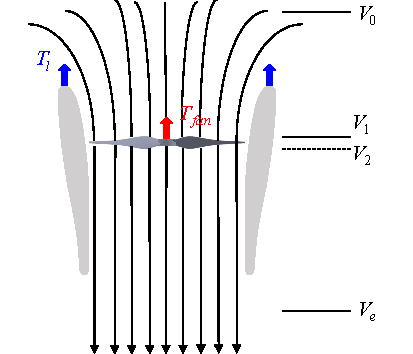
\includegraphics[scale=1]{Fig/轴流管道模型.pdf}
		\caption{\label{轴流管道模型}轴流状态的空气动力学}
	\end{minipage}%
\end{figure}

假设风扇旋转时的桨盘面积为$S$,涵道扩压比为$\sigma_d$,$\sigma_d$表示涵道下方出口横截面面积与桨盘面积$S$之比。那么根据质量守恒有:
\begin{equation}
    \sigma_dSV_e=SV_2=SV_1
    \label{eq_17}
\end{equation}

设空气密度为$\rho$,单位时间内通过涵道风扇的气流总质量为$\dot{m}_{air}$。一方面,根据动量定理可知,涵道风扇对气流施加的总作用力等于单位时间内气流通过风扇的动量变化率:
\begin{equation}
    T_{fan}=\dot{m}_{air}(V_e-V_0)=\rho S V_1(V_e-V_0)
    \label{eq_18}
\end{equation}
另一方面,气体动能的变化量等同于涵道风扇输送给气体的功率:
\begin{equation}
    \frac{1}{2}\dot{m}_{air}V_e^2-\frac{1}{2}\dot{m}_{air}V_0^2=T_{fan}V_1
    \label{eq_19}
\end{equation}
结合\eqref{eq_17}、\eqref{eq_18}和\eqref{eq_19},可以得到涵道出口风速$V_e$\cite{pereiraHoverWindtunnelTesting2008}:
\begin{equation}
    V_e=\frac{V_0}{2}+\sqrt{\left(\frac{V_0}{2}\right)^2+\frac{T_{fan}}{\sigma_d\rho S}}    \label{eq_20}
\end{equation}
定义涵道风扇的诱导速度为$V^{\prime}=V_1-V_0$,那么结合\eqref{eq_17}和\eqref{eq_20}可以得到:
\begin{equation}
    \begin{aligned}
    V^{\prime}&=\sigma_dV_e-V_0 \\
    &=\left(\frac{\sigma_d}{2}-1\right)V_0+\sqrt{\left(\frac{V_0\sigma_d}{2}\right)^2+\frac{T_{fan}\sigma_d}{\rho S}}
    \label{induced velocity}
    \end{aligned}
\end{equation}
涵道出口处的气流速度$V_e$和涵道风扇的诱导速度$V^{\prime}$将在后续的空气动力学分析中发挥重要作用,包括涵道翼型上产生的附加阻力的计算、控制舵面上的力与力矩的计算以及固定气动面扭矩的计算等。

关于涵道风扇产生的拉力$T_{p}$、侧向拉力$T_{l}$和扭矩$\boldsymbol{M}_{fan}^b$的计算,由下式给出\cite{luoNumericalAnalysisWind2024a}:
\begin{equation}
    \begin{aligned}
        T_{p}&=\rho S \Omega^2R^2 C_{p}\\
        T_{l}&=\rho S \Omega^2R^2 C_{l}\\
        \boldsymbol{M}_{fan}^b&=\rho S \Omega^2 R^3C_{q}
    \end{aligned}
    \label{eq_21}
\end{equation}
其中$\Omega$是涵道风扇的旋转角速度,$R$是涵道风扇的旋转半径,$C_{p}$、$C_{l}$和$C_{q}$分别是涵道风扇的拉力系数、侧向推力系数和扭矩系数。这三个系数与环境风速、飞机姿态等因素有关,难以用简单的解析式来表示。大部分文献都采用数值分析方法来测定\cite{iiiNondimensionalModelingDuctedFan2012,choiStaticAnalysisSmall2012,luoNumericalAnalysisWind2024a}。

由于$\rho$、$S$、$R$均为常数,涵道风扇产生的总的拉力$\boldsymbol{F}_{fan}^b$和扭矩$\boldsymbol{M}_{fan}^b$仅在机体系下的${\boldsymbol{O}_b}-{\boldsymbol{Z}_b}$轴产生效果,所以可以近似简化为以下形式\cite{choiStaticAnalysisSmall2012,manzoorCompositeObserverbasedRobust2023}:
\begin{align}
            \boldsymbol{F}_{fan}^b=\begin{bmatrix}0 \\ 0 \\
                -k_{fan}\Omega^2
            \end{bmatrix},\quad    
            \boldsymbol{M}_{fan}^b=\begin{bmatrix}0 \\ 0 \\
            -k_{q}\Omega^2
            \end{bmatrix}    \label{eq_22}
\end{align}
其中$k_{fan}$和$k_{q}$均为常系数,可采用数值分析方法近似测定。
\subsection{机身动力学}

涵道机身的气动阻力和力矩源于机身与气流错综复杂的相互作用。当无人机在空中飞行时,周围的气流会以一定的速度与涵道机身表面接触。这种相互碰撞、摩擦,形成了阻碍飞机前进的气动阻力。同时,由于气流在机身不同部位的速度和压强分布不均匀,会对机身产生一个使它绕某一轴转动的趋势,这便是气动力矩。根据空气动力学原理,气动阻力与飞机与气流相对速度的平方大致成正比关系。而且速度的变化还会影响气流在机身周围的流动形态,使得气动力矩也发生相应变化。另外,沿机体轴方向的横截面积同样是影响气动阻力和力矩的重要因素。较大的横截面积意味着气流与机身的接触面积更大,气流在流经机身时受到的阻碍也会增加。由于DFUAV的外部由涵道体包裹,因此横截面积较大,更会加剧这一过程。

定义空速向量$\boldsymbol{V}_a^b= [ u_r \quad v_r \quad w_r ]^T$为机体相对于气流的速度在机体系的投影,标量表示为$V_a$,空速与环境风速有关。当环境风速$W^e$为零时,$\boldsymbol{V}_a^b=\boldsymbol{V}^b$。在机身产生的力与力矩可表示为\cite{johnsonModelingControlFlight2006b,choiStaticAnalysisSmall2012}:
\begin{gather}
    \boldsymbol{F}_{aero}^b=-\frac{1}{2}\rho
    \begin{bmatrix}
    C_{D,x}S_xu_r|u_r| \\
    C_{D,y}S_yv_r|v_r| \\
    C_{D,z}S_zw_r|w_r|
    \end{bmatrix}\label{eq_22.5}\\
    \boldsymbol{M}_{aero}^b=\frac{1}{2}\rho
    \begin{bmatrix}
    C_{D,y}S_yv_r|v_r| \\
    -C_{D,x}S_xu_r|u_r| \\
    0
    \end{bmatrix}l_{a}
    \label{eq_23}
\end{gather}
其中$C_{D,x}$、$C_{D,y}$和$C_{D,z}$分别是机身沿机体系三个轴方向的气动阻力系数,$S_x$、$S_y$和$S_z$分别是机身沿机体系三个轴方向的横截面积,$l_{a}$表示DFUAV的机身空气动力中心和其重心之间的距离。

由$\boldsymbol{M}_{aero}^b$的表达式可以看出,机身气动力矩不会影响机体系下的${\boldsymbol{O}_b}-{\boldsymbol{Z}_b}$轴,暗含DFUAV的空气动力中心和其重心之间的距离在${\boldsymbol{O}_b}-{\boldsymbol{X}_b}$轴和${\boldsymbol{O}_b}-{\boldsymbol{Y}_b}$轴上的分量为零,这是由于DFUAV的几何对称特性所导致的。

\subsection{涵道动力学}

类似直升机旋翼的经典建模方法,本小节基于不可压缩的定常流动假设建立升力$L$-阻力$D$模型来估算空速施加在涵道环翼上的气动力与力矩\cite{johnsonModelingControlFlight2006b},如图\ref{非轴流状态}所示。

\begin{figure}[htbp]
	\centering
	\begin{minipage}[c]{1\textwidth}
		\centering
		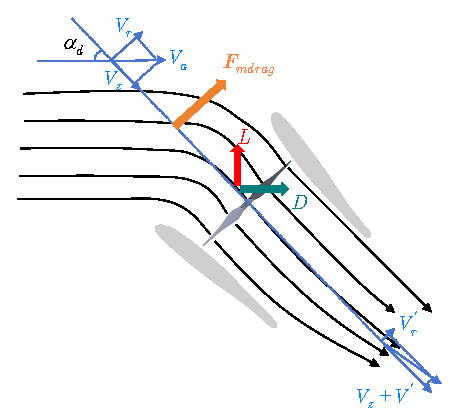
\includegraphics[scale=1]{Fig/非轴流状态.pdf}
		\caption{\label{非轴流状态}非轴流状态(前飞时)的空气动力学}
	\end{minipage}%
\end{figure}

假设$\gamma$代表在机体系${\boldsymbol{O}_b}-{\boldsymbol{X}_b}{\boldsymbol{Y}_b}$平面内的角度度量,$\boldsymbol{i}$和$\boldsymbol{j}$分别表示沿着机体系${\boldsymbol{O}_b}-{\boldsymbol{X}_b}$轴和${\boldsymbol{O}_b}-{\boldsymbol{Y}_b}轴$的单位向量。那么在${\boldsymbol{O}_b}-{\boldsymbol{X}_b}{\boldsymbol{Y}_b}$平面内的单位向量和速度向量可以表示为:
\begin{align}
    \boldsymbol{e}_{r}&=\cos\gamma\boldsymbol{i}+\sin\gamma\boldsymbol{j} \label{eq_24}\\
    \boldsymbol{V}_{xy}&=-u_r\boldsymbol{i}-v_r\boldsymbol{j} \label{eq_25}
\end{align}
由于式\eqref{eq_25}中的速度表示机体相对于气流的速度,为表示气流相对于机体的速度需要加负号。为方便表示,假设在涵道周围沿${\boldsymbol{O}_b}-{\boldsymbol{Z}_b}$轴方向的速度分量是恒定的。那么径向速度${V}_{r}(\gamma)$作为$\gamma$的函数可以写为:
\begin{equation}
    V_r(\gamma)=\boldsymbol{V}_{xy}\cdot{\boldsymbol{e}}_r=-u_r\cos\gamma-v_r\sin\gamma    \label{eq_26}
\end{equation}
气流速度在${\boldsymbol{O}_b}-{\boldsymbol{Z}_b}$轴方向相对于机体的速度分量$V_z(\gamma)$可以表示为:
\begin{equation}
    V_z(\gamma)=-w_r   \label{eq_27}
\end{equation}
其中诱导速度$V^{\prime}$于式\eqref{induced velocity}中定义。

现在,涵道周围的动态压力$q_d(\gamma)$和迎角$\alpha_d(\gamma)$可以如下计算:
\begin{equation}
    \begin{aligned}
        q_d(\gamma)&=\frac{1}{2}\rho\left(V_r^2+V_z^2\right)\\
        \alpha_d(\gamma)&=\tan^{-1}\left(\frac{V_r}{V_z}\right)
    \label{eq_28}
    \end{aligned}
\end{equation}
根据式\eqref{eq_28}进一步可以表示出涵道周围单位展长的升力$l(\gamma)$和阻力$d(\gamma)$及其在每个机体轴的分量:
\begin{equation}
        l(\gamma)=C_{l,d}(\alpha_d)c_dq_d, \quad
        d(\gamma)=C_{d,d}(\alpha_d)c_dq_d
    \label{eq_29}
\end{equation}
\begin{equation}
        \begin{aligned}
            \Rightarrow
        l_{x}(\gamma)&=l(\gamma)\cos\alpha_d\cos\gamma,\quad d_x(\gamma)=d(\gamma)\sin\alpha_d\cos\gamma \\
        l_{y}(\gamma)&=l(\gamma)\cos\alpha_d\sin\gamma,\quad d_y(\gamma)=d(\gamma)\sin\alpha_d\sin\gamma \\
        l_{z}(\gamma)&=-l(\gamma)\sin\alpha_d,\quad d_z(\gamma)=d(\gamma)\cos\alpha_d
        \label{eq_30}
    \end{aligned}
\end{equation}
式\eqref{eq_29}中$C_{l,d}$、$C_{d,d}$分别是涵道翼型的升力曲线和阻力曲线,均与迎角$\alpha_d(\gamma)$有关。$c_d$是涵道翼型的弦长。将式\eqref{eq_30}中的各轴向分量沿该轴方向积分便可得到每个轴的气动升力和阻力,如$x$轴方向:
\begin{equation}
    L_x=R\int_0^{2\pi}l_x(\gamma)d\gamma, \quad
    D_x=R\int_0^{2\pi}d_x(\gamma)d\gamma
    \label{eq_31}
\end{equation}

除气动升力和阻力外,DFUAV前飞时(非轴流状态)在涵道上还会产生附加的阻力(即动量阻力$\boldsymbol{F}_{mdrag}$\cite{choiStaticAnalysisSmall2012})。如图\ref{非轴流状态}所示,由于涵道体的遮挡,气流的径向速度$V_r$分量在进入涵道体后迅速衰减为$V_r^\prime$,因此导致径向气体动量的变化,从而产生附加的阻力。该阻力可以通过进入涵道的空气质量流量和飞行速度来表示:
\begin{equation}
    \boldsymbol{F}_{mdrag}=-V^\prime\rho{S}
    \begin{bmatrix}u_r \\v_r \\0
    \end{bmatrix}
    \label{eq_32}
\end{equation}

侧风作用于涵道结构形成的的非对称升力分布同样会产生力矩,假定该力矩与侧风引起的动态压力为近似线性关系,那么可量化为:
\begin{equation}
    \boldsymbol{M}_{lip}=C_{duct}\rho{R}
    \begin{bmatrix}v_r|v_r| \\-u_r|u_r| \\0\end{bmatrix}
    \label{eq_33}
\end{equation}
其中,$C_{duct}$是常系数。该系数最初可根据iSTAR\cite{flemingImprovingControlSystem}的实验数据估算,随后需要结合实际情况调整。

综合\eqref{eq_31}、\eqref{eq_32}、\eqref{eq_33},在涵道翼型上产生的力与力矩可以表示为\cite{johnsonModelingControlFlight2006b,choiStaticAnalysisSmall2012}:
\begin{align}
    \boldsymbol{F}_{duct}^b=
    \begin{bmatrix}
    L_x+D_x \\
    L_y+D_y \\
    L_z+D_z
    \end{bmatrix}+\boldsymbol{F} _{mdrag}\label{eq_33.5}\\
    \boldsymbol{M}_{duct}^b=
    \begin{bmatrix}
    L_xl_d \\
    L_yl_d \\
    0
    \end{bmatrix}+\boldsymbol{M}_{lip}
    \label{eq_34}
\end{align}
其中$l_d$表示DFUAV的重心与涵道空气动力中心之间的距离。

\subsection{控制舵面动力学}

涵道底部的控制舵面是DFUAV的主要控制机构,在飞行过程中控制舵面的运动会产生气动力和力矩,这些力矩是造成DFUAV进行滚转、俯仰、偏航姿态变化的主要原因。如图\ref{控制舵面}所示,本文研究的DFUAV配置有四片交叉排列的控制舵面,定义机体系${\boldsymbol{O}_b}-{\boldsymbol{X}_b}$轴正方向下方位置对应的控制舵面为1号舵,从上往下按照顺时针方向依次编号为2、3、4号舵。1、3号舵的同向运动用于产生滚转力矩,2、4号舵的同向运动用于产生俯仰力矩,4个舵的共同差动用于产生偏航力矩。定义控制舵面的偏转角度为$\boldsymbol{\delta}=[\delta_1\quad\delta_2\quad\delta_3\quad\delta_4]^T$,分别对应4个控制舵面。规定向右偏转为正方向,零位点保持与机体系${\boldsymbol{O}_b}-{\boldsymbol{Z}_b}$轴平行。

\begin{figure}[htbp]
	\centering
	\begin{minipage}[c]{0.5\textwidth} % minipage将页面划分为0.5\textwidth
		\centering
		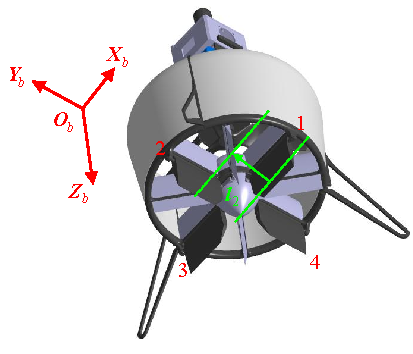
\includegraphics[scale=1]{Fig/控制舵面.pdf}
	\end{minipage}%
	\begin{minipage}[c]{0.5\textwidth}
		\centering
		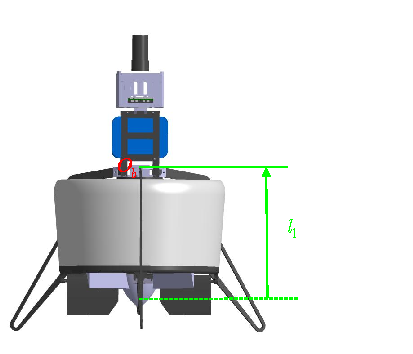
\includegraphics[scale=1]{Fig/力臂.pdf}
	\end{minipage}
    \caption{\label{控制舵面}控制舵面及力臂示意图}
\end{figure}

在涵道风扇滑流中,控制舵面的偏转而产生的升力与机体系${\boldsymbol{O}_b}-{\boldsymbol{Z}_b}$轴垂直,且与转角$\delta_i$的平方成正比\cite{pflimlinModelingAttitudeControl2010a}:
\begin{equation}
    F_i=k_\delta{V_e}^2\delta_i \quad i=1,2,3,4
    \label{eq_35}
\end{equation}
其中$k_\delta$是正的常数,表示控制舵面升力系数。${V_e}$为涵道出口风速,由式\eqref{eq_20}给出。

因此,由控制舵面产生的合力与合力矩可以表示为\cite{pflimlinModelingAttitudeControl2010a,manzoorCompositeObserverbasedRobust2023}:
    \begin{gather}
    \boldsymbol{F}_{vane}^b=\begin{bmatrix}
    F_4-F_2 \\ F_1-F_3 \\ 0 
    \end{bmatrix}     \label{eq_35.5}\\
    \boldsymbol{M}_{vane}^b=\begin{bmatrix}
        -l_1(F_1-F_3) \\ l_1(F_4-F_2) \\ l_2(F_1+F_2+F_3+F_4) 
    \end{bmatrix}
    \label{eq_36}
    \end{gather}
式\eqref{eq_36}中的$l_1$和$l_2$分别为涵道的力臂,如图\ref{控制舵面}所示。事实上,控制舵面的偏转角仅在DFUAV的失速迎角的范围内才有效果\cite{9787121348440000},超出该范围后,姿态将难以控制。因此需要对偏转角度进行限幅处理:
\begin{equation}
    -\delta_m\leq\delta_{i}\leq\delta_m,\quad i=1,2,3,4
    \label{eq_37}
\end{equation}
对于本文研究的DFUAV,限幅值$\delta_m$取$40^\circ$。

\subsection{陀螺力矩与固定气动面反扭矩}

涵道风扇在高速旋转时,DFUAV整体会呈现出类似陀螺的特性。根据角动量守恒定律,当涵道风扇的旋转轴在外力影响下发生偏移时,为了维持整个系统角动量的守恒,涵道风扇会产生一个特殊的反作用力矩。该力矩垂直于旋转轴的偏移方向,试图将旋转轴拉回到原来的方向,从而抵抗外力对旋转状态的干扰。这种作用力矩即为陀螺力矩,其大小与风扇的转动惯量和旋转的角速度有关。转动惯量体现了涵道风扇抵抗转动状态改变的能力,它取决于风扇的质量分布以及形状等因素。角速度反映了风扇旋转的快慢程度。当风扇以较高的角速度旋转时,角动量也较大,为了维持角动量而产生的陀螺力矩也越大。所以有:
\begin{equation}
    \boldsymbol{M}_{gyro}^b=J_{fan}\Omega
    \begin{bmatrix}
    -q \\ p \\ 0
    \end{bmatrix}
    \label{eq_38}
\end{equation}
其中$J_{fan}$为涵道风扇的转动惯量。

固定气动面是指位于涵道内部,涵道风扇下方的固定装置。其特殊的外形结构用于在涵道风扇滑流中产生反扭矩来抵消DFUAV单一风扇产生的风扇扭矩$\boldsymbol{M}_{fan}^b$,涵道内部流场示意图如图\ref{固定气动面}所示。经过涵道风扇加速后的气流在经过固定气动面时会发生偏转,进而在气动面上产生作用力和力矩。固定气动面的反扭距效应可以近似表示为\cite{1020333010.nh}:
\begin{equation}
    \boldsymbol{M}_{flap}^b=V_e^2\varphi_0
    \begin{bmatrix}
    0 \\0 \\d_{af}
    \end{bmatrix}
    +V_e\Omega
    \begin{bmatrix}
    0 \\0 \\d_{ds}
    \end{bmatrix}
    \label{eq_39}
\end{equation}
其中$\varphi_0$是固定气动面的安装角,$d_{af}$和$d_{ds}$均为常数。

\begin{figure}[htbp]
	\centering
	\begin{minipage}[c]{1\textwidth} 
		\centering
		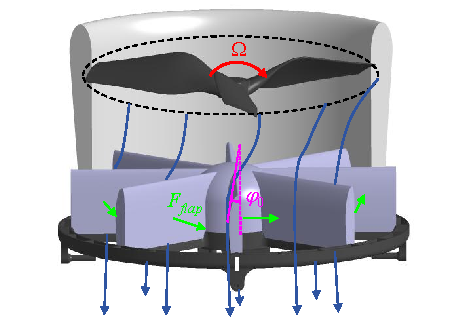
\includegraphics[scale=1]{Fig/固定气动面.pdf}
	\end{minipage}%
    \caption{\label{固定气动面}涵道内部流场示意图}
\end{figure}

经过恰当的设计,固定气动面产生的反扭距$\boldsymbol{M}_{flap}^b$可以抵消大部分的风扇扭矩$\boldsymbol{M}_{fan}^b$。在实践过程中很难达到理想情况,即$\boldsymbol{M}_{flap}^b + \boldsymbol{M}_{fan}^b = \boldsymbol{0}$,所以剩余的力矩部分将由控制舵面的偏置产生偏航力矩来进行补偿。

\section{系统建模总结}

DFUAV的输入变量包括涵道风扇的转速$\Omega$和四个控制舵面的偏转角$\delta_i$,作为动力核心的涵道风扇通过转速调节产生主推力,四片分布式气动舵面通过独立偏转生成三维控制力矩。系统的输出为状态变量,其中包括DFUAV在地面坐标系下的位置$\boldsymbol{P}^{e}=[{x}^{e} \quad {y}^{e} \quad {z}^{e}]^{T}$、地面坐标系下的速度$\boldsymbol{V}^{e}=[{v}^{e}_{x} \quad {v}^{e}_{y} \quad {v}^{e}_{z}]^{T}$、姿态角$\boldsymbol{\eta}=[\varphi \quad \theta \quad \psi]^T$以及机体坐标系下的角速度$\boldsymbol{\omega}^b=[p \quad q \quad r]^T$。结合DFUAV的飞行控制刚体模型和力与力矩的分析,可以推导出DFUAV的非线性动态方程,如下所示:

位置动态方程:
\begin{equation}
    \begin{aligned}
        \dot{x}^{e}&=v_x^e\\
        \dot{y}^{e}&=v_y^e\\
        \dot{z}^{e}&=v_z^e
    \end{aligned}
    \label{eq_40}
\end{equation}

速度动态方程:
\begin{equation}
    \begin{aligned}
        \dot{v}_{x}^{e} & =\frac{1}{m}\Bigg\{ (\cos{\theta}\cos{\psi}) 
        \cdot\left[-\frac{1}{2}\rho C_{D,x}S_xu_r|u_r|+L_x+D_x - V'\rho S u_r + k_\delta V_e^2(\delta_4 - \delta_2)\right] \\
        & \quad+ (\sin{\varphi}\sin{\theta}\cos{\psi}-\cos{\varphi}\sin{\psi}) \\
        & \quad\cdot\left[-\frac{1}{2}\rho C_{D,y}S_yv_r|v_r|+L_y+D_y - V'\rho S v_r + k_\delta V_e^2(\delta_1 - \delta_3)\right] \\
        & \quad+ (\cos{\varphi}\sin{\theta}\cos{\psi}+\sin{\varphi}\sin{\psi}) \\
        & \quad\cdot\left[-k_{fan}\Omega^2-\frac{1}{2}\rho C_{D,z}S_zw_r|w_r|+L_z+D_z\right]
        \Bigg\}
        \\
        \dot{v}_{y}^{e} & =\frac{1}{m}\Bigg\{ (\cos{\theta}\sin{\psi}) \cdot\left[-\frac{1}{2}\rho C_{D,x}S_xu_r|u_r|+L_x+D_x - V'\rho S u_r + k_\delta V_e^2(\delta_4 - \delta_2)\right] \\
        & \quad+ (\sin{\varphi}\sin{\theta}\sin{\psi}+\cos{\varphi}\cos{\psi}) \\
        & \quad\cdot\left[-\frac{1}{2}\rho C_{D,y}S_yv_r|v_r|+L_y+D_y - V'\rho S v_r + k_\delta V_e^2(\delta_1 - \delta_3)\right] \\
        & \quad+ (\cos{\varphi}\sin{\theta}\sin{\psi}-\sin{\varphi}\cos{\psi}) \\
        & \quad\cdot\left[-k_{fan}\Omega^2-\frac{1}{2}\rho C_{D,z}S_zw_r|w_r|+L_z+D_z\right]
        \Bigg\}
        \\
        \dot{v}_{z}^{e} & =\frac{1}{m}\Bigg\{ -\sin{\theta}\cdot\left[-\frac{1}{2}\rho C_{D,x}S_xu_r|u_r|+L_x+D_x - V'\rho S u_r + k_\delta V_e^2(\delta_4 - \delta_2)\right] \\
        & \quad+ (\sin{\varphi}\cos{\theta})\cdot\left[-\frac{1}{2}\rho C_{D,y}S_yv_r|v_r|+L_y+D_y - V'\rho S v_r + k_\delta V_e^2(\delta_1 - \delta_3)\right] \\
        & \quad+ (\cos{\varphi}\cos{\theta}) \cdot\left[-k_{fan}\Omega^2-\frac{1}{2}\rho C_{D,z}S_zw_r|w_r|+L_z+D_z\right]
        \Bigg\}+g
    \end{aligned}
    \label{eq_41}
\end{equation}

姿态动态方程:
\begin{equation}
    \begin{aligned}
        \dot{\varphi}&=p+\sin{\varphi}\tan{\theta}q+\cos{\varphi}\tan{\theta}r\\
        \dot{\theta}&=\cos{\varphi}q-\sin{\varphi}r\\
        \dot{\psi}&=\frac{\sin{\varphi}}{\cos{\theta}}q+\frac{\cos{\varphi}}{\cos{\theta}}r
    \end{aligned}
    \label{eq_42}
\end{equation}

角速度动态方程:
\begin{equation}
    \begin{aligned}
        \dot{p}  &=\frac{1}{J_x}\Bigg\{ (J_y-J_z)qr+
        \bigg[\frac{1}{2}\rho{l_a} C_{D,y}S_yv_r|v_r|+L_xl_d+C_{duct}\rho{R}
        v_r|v_r| \bigg.\\
        & \quad\bigg.- l_1k_\delta V_e^2(\delta_1 - \delta_3)-J_{fan}\Omega{q}\bigg]\Bigg\} \\
        \dot{q}  &=\frac{1}{J_y}\Bigg\{ (J_z-J_x)pr+
        \bigg[-\frac{1}{2}\rho{l_a} C_{D,x}S_xu_r|u_r|+L_yl_d+C_{duct}\rho{R}
        u_r|u_r| \bigg.\\
        & \quad\bigg.+ l_1k_\delta V_e^2(\delta_4 - \delta_2)+J_{fan}\Omega{p}\bigg]\Bigg\} \\
        \dot{r}  &=\frac{1}{J_z}\Bigg\{ (J_x-J_y)pq+
        \left[-k_q\Omega^2 +l_2k_\delta V_e^2(\delta_1 + \delta_2 + \delta_3 + \delta_4)\right.\\
        & \quad\left.+V_e^2\varphi_0d_{af}+V_e\Omega{d_{ds}}\right]
        \Bigg\}
    \end{aligned}
    \label{eq_43}
\end{equation}

本文通过物理实验与计算流体力学(Computational Fluid Dynamics,CDF)相结合的方法近似测得试验样机的非线性系统动态方程相关参数,如表\ref{DFUAV_parameters}所示。

\begin{table}
	\caption{\label{DFUAV_parameters}涵道模型参数}
	\centering
	\small 
	\begin{tabular}{cccc}
		\hline 
		参数符号 & 数值                & 参数符号 & 数值                 \tabularnewline
		\hline 
		$m(kg)$   & $1.85$ 		     & $J_x,J_y(kg\cdot{m}^2)$   & $0.0149         $ \tabularnewline
		$J_z(kg\cdot{m}^2)$   & $0.005516$ & $\sigma_d$   & $0.7$ \tabularnewline
        $\rho(kg/m^3)$   & $1.225$ & $R(m)$   & $0.114$ \tabularnewline
        $k_{fan}$   & $9.9796\times10^{-6}$ & $k_q$   & $1.1334\times10^{-7}$ \tabularnewline
        $C_{D,x}$   & $0.43213$ & $C_{D,y}$   & $0.43213$ \tabularnewline
        $C_{D,z}$   & $0.13421$ & $S_x,S_y,S_z(m^2)$   & $0.04$ \tabularnewline
        $l_a(m)$   & $0.1121$ & $C_{duct}$   & $0.78497$ \tabularnewline
        $k_{\delta}$   & $0.0073$ & $J_{fan}(kg\cdot{m}^2)$   & $3.7\times10^{-5}$ \tabularnewline
        $d_{af}$   & $0.01495$ & $d_{ds}$   & $0.01495$ \tabularnewline
        $l_1(m)$   & $0.1708$ & $l_2(m)$   & $0.0066$ \tabularnewline
		\hline 
	\end{tabular}
\end{table}

由DFUAV的非线性动态方程可知,DFUAV的飞行动态呈现为一个高度非线性的多变量耦合系统,系统内各状态变量之间存在着复杂且紧密的相互作用。若要将所有相关变量纳入考量,控制算法的设计工作将尤为棘手。因此在具体实践过程中,可以根据实际情况合力简化模型,有针对性地忽略部分影响较小的因素,保留决定系统宏观特性的主干动力学。然而,模型简化意味着信息缺失,对于未被建模的动态特性(如突然的阵风扰动、机械结构磨损等)以及因简化模型而产生的误差,则可通过鲁棒性的飞行控制算法来进行补偿。

\section{本章小结}

本章主要介绍了试验样机的系统组成并围绕DFUAV的系统建模展开系统性研究。

首先介绍了所使用的试验样机的整体系统组成,明确了各个部分的功能和相互关系,为后续建模及飞行实验奠定物理基础。

接着介绍了坐标系和姿态表示方法,建立了地面坐标系与机体坐标系的转换关系,并根据实际约束采用了‘Z-Y-X’旋转顺序的欧拉角姿态表示方法为飞行控制系统的建模提供了必要的数学分析工具。

在DFUAV的飞行控制刚体模型构建中,结合牛顿-欧拉方程推导出六自由度非线性动力学方程,完整表征平动与转动状态的关系。

并从涵道风扇、机身、涵道翼型、控制舵面和固定气动面等多个方面分析了施加在上面的力与力矩,揭示了各类作用力和控制力矩对飞行器姿态和运动的动态影响。

最后建立了DFUAV的完整的非线性动态方程,本章建立的参数化模型为后续控制算法设计、仿真验证及飞行试验提供了理论框架与数值分析基础。
